
\documentclass[a4paper,11pt]{article}

\usepackage{fontspec}
\setmainfont{Calibri}

\linespread{1}

\setlength{\oddsidemargin}{0cm}
\setlength{\evensidemargin}{0cm}
\setlength{\textheight}{23cm}
\setlength{\textwidth}{16cm}

\usepackage{amssymb,mathrsfs,algorithmic,algorithm,multirow}
\usepackage{amsmath,amsbsy,graphicx,color,url,natbib}
\usepackage{ccaption}
\setlength{\bibsep}{0.0pt}

\newcommand{\bm}{\mathbf}
\newcommand{\bs}{\boldsymbol}
\newcommand{\mt}{\mathrm}
\newcommand{\nind}{\noindent}

\usepackage{fancyhdr}
\newcommand{\tstamp}{\today}   
\lhead[\fancyplain{}{\rightmark}]       {\fancyplain{}{}}
\rhead[\fancyplain{}{\rightmark}]       {\fancyplain{}{}}
\chead[\fancyplain{}{\centermark}]       {\fancyplain{}{ENGM214 -- Process Modelling and Simulation} }
\pagestyle{fancyplain}

\usepackage{amsthm}
\theoremstyle{definition}
\newtheorem{exmp}{Example}[section]

\title{\vspace{-2cm} Lecture 2 -- Principles for constructing mechanistic models}

\author{Tao Chen\\
{\small \emph{Department of Chemical \& Process Engineering, University of Surrey, UK}}\\
{\small (email: \texttt{t.chen@surrey.ac.uk}; \hspace{0.5cm} updated on \today )}
}
\date{}

\begin{document}
\maketitle

%\tableofcontents
\vspace{-0.5cm}


\section{The general procedure for building models}

The general procedure is outlined in Fig. \ref{fig:procedure}.
The important considerations have been well covered in the lecture slides.
Here we only stress a few points.

\begin{figure} [!h]
 \begin{center}
	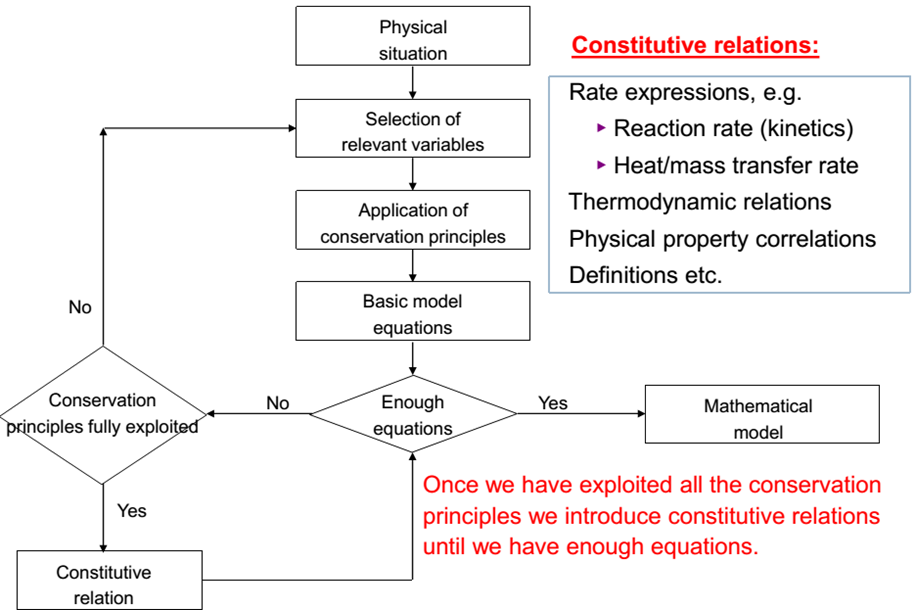
\includegraphics[width=.9\textwidth]{procedure}\\
 \end{center}
 \caption{Overview of the procedure for building models.} 
 \label{fig:procedure}
\end{figure}

\begin{itemize}
	\item \textbf{Modelling has a purpose.}  The purpose will determine
		the complexity of the model, e.g. dynamic vs steady-state,
		lumped parameter vs distributed parameter, mechanistic vs data-driven model,
		the scale at which	the model should be developed (e.g. microscopic molecular scale vs
		macroscopic process scale), etc.
	\item \textbf{All models are wrong, some are useful.} We should never aim to
		build a model that reflects 100\% reality, for this is not possible.
		Instead we should assess whether the model is ``useful'' for the purpose of modelling,
		and clearly state the assumptions/simplifications in the model.
	\item \textbf{Modelling is both a science and an art.} Inevitably modelling involves
		subjective judgements in terms of what mechanisms should be considered, what variables
		are important, what assumptions should be made, etc. The same problem could be
		modelled in many different ways, and the choice is not ``black or white'' and requires
		modeller's experience.
	\item \textbf{Mechanistic models usually contain two parts}: conservation equations
		and constitutive relations. This will be elaborated in Lecture 3.
\end{itemize}


\section{The concept of degrees of freedom}

Degrees of freedom (DoF) is about the number of equations vs the number of variables
in a model. Consider the following model described by algebraic equations:
\[  x_3 - 2 x_1 + x_2 = 2 \]
\[  x_4 + x_1 - 3 x_2 = 2 \]
\[  x_5 + x_1 + x_2 = 4 \]
Here the number of equations is 3 and the number of variables is 5. We could re-arrange
the equations as follows (one of many possible ways):
\[  x_3 = 2 x_1 - x_2 + 2 \]
\[  x_4 = -x_1 + 3 x_2 + 2 \]
\[  x_5 = -x_1 - x_2 + 4 \]
and by specifying any value for $x_1$ and $x_2$, the other three variables
($x_3$, $x_4$ and $x_5$) can be determined from the above equations.
In this case $x_1$ and $x_2$ are called \emph{independent variables}, and the other
variables \emph{dependent variables}. We say the DoF of this system is 2.

In general, DoF (we also use $N_{DF}$ as notation) is calcuated by
\[ N_{DF} = NV - NE \]
where $NV$ is the number of variables and $NE$ the number of \emph{independent equations}.
An equation is independent of other equations if it cannot be derived from the other equations.
For example, include another equation $2 x_4 + 2 x_1 - 6 x_2 = 4$ to
\[  x_3 - 2 x_1 + x_2 = 2 \]
\[  x_4 + x_1 - 3 x_2 = 2 \]
\[  x_5 + x_1 + x_2 = 4 \]
will not change $N_{DF}$, because the new equation can be obtained from the second equation
(multiplying both sides by 2).

For a given equation system,
\begin{itemize}
	\item $N_{DF}<0$: The system is over-specified, no solution exists. (Although no solution exists,
		the technique of mathematical optimisation could be used to find the value of the variables
		by optimising a certain objective function. This topic is discussed in ``ENGM072 -- Optimisation and Decision Making''.)
	\item $N_{DF}=0$: The system is fully specified; it is possible to obtain an unique set of solution and simulation is possible.
	\item $N_{DF}>0$: The system is under-specified, no unique solution exists; some variables must be specified,
		or more equations added, in order to perform simulation.
\end{itemize}

\section{A modelling example -- thermodynamics}

The modelling example has been well explained in the slides and thus will not be repeated here.
However, I'd stress the importance of revisit the key concepts and results of thermodynamics,
which is used in various places in this module.
At the minumum, you are recommended to read Appendix A and B of the book ``Chemical and Energy Process Engineering'' by Sigurd Skogestad
(check the reading list of ENGM214 for access to this book), which provide very good review of thermodynamics.
More detailed treatment of thermodynamics can be found in numerous textbooks, e.g. \citep{Smith2004} which has
very comprehensive screencasts provided by the University of Colorado Boulder 
(\url{https://sites.google.com/a/learncheme.com/learncheme/screencasts/thermodynamics/textbook-SVNA-7th}).


\begin{thebibliography}{2}
\vspace{-0.4cm}
\bibitem[{Hangos(2001)}]{Hangos2001}
	Hangos KM, Cameron IT, 2001. Process Modelling and Model Analysis, Academic Press: London.

\bibitem[{Smith(2004)}]{Smith2004}
	Smith JM, van Ness HC, Abbott MM, 2004. Introduction to Chemical Engineering Thermodynamics, 7th edition, McGraw-Hill.
\end{thebibliography}

\end{document}


